\documentclass[inf, h]{pjatkThesis}
\usepackage{times}
\usepackage[polish]{babel}
\usepackage[utf8]{inputenc}
\usepackage{gensymb}
\usepackage{graphicx}
\usepackage{makeidx}
\usepackage{lipsum}
\usepackage{color}
\usepackage{xcolor}
\usepackage{listings}
\usepackage{caption}
\usepackage{minted}



\author{Patryk Ptasiński}
\album{Numer albumu 10623}
\title{Nawigacja w warunkach miejskich przy użyciu danych o lokalizacjach sieci WIFI}
\type{Praca inżynierska}
\supervisor{dr. inż Michał Tomaszewski}
\location{Warszawa}
\date{czerwiec 2017}

% do wydruków
%\usepackage[T1]{fontenc}
%\usepackage{lmodern,cmap}
%\usepackage[none]{hyphenat}


\begin{document}

\tableofcontents
%\listoffigures
%\listoftables

% zmiana nazwy abstraktu

\begin{abstract}
W swojej pracy przedstawię specyfikację technologi bezprzewodowej transmisji danych zwaną WIFI. Omówię problemy i wyzwania przy zbieraniu informacji o sieciach bezprzewodowych. Zanalizuję zebrane oraz publicznie dostępne dane o lokalizacjach sieci WiFi. 
\end{abstract}
%\pagenumbering{gobble}
\pagenumbering{arabic}
\baselineskip=22pt

\chapter*{Wprowadzenie}
\label{ch:wprowadz}

Skąd pomysł na badanie tematu sieci WiFi? Technologia ta już rozprzestrzeniła się na całym Świecie z ogromnym sukcesem. Więc można by postawić tezę, że w tym obszarze nie czeka na nas nic interesującego. Nic bardziej mylnego! Dopiero, teraz gdy sieci bezprzewodowe się rozprzestrzeniły na skalę masową, to możemy badać oraz projektować i tworzyć rozwiązania w oparciu na popularności tej technologii. Gdy wejdziemy do przeciętnego mieszkania wielopiętrowego bloku, to w zasięgu są dziesiątki, a czasem nawet setki bezprzewodowych sieci. Gdyby zapisać lokalizację tych wszystkich sieci bezprzewodowych, to utworzymy system, który umożliwia użytkownikom względne pozycjonowanie. W mojej pracy postaram się odpowiedzieć na pytanie, jak zbudować i korzystać z takiego systemu.

\chapter{Część teoretyczna}

W tym rozdziale zostaną przedstawione technologie, proces projektowania aplikacji internetowej oraz aplikacji mobilnej, odwołam się do teorii, na których podstawie zostaną zaimplementowane algorytmy w obydwu aplikacjach. Na koniec postawię tezę, którą zweryfikuję w części praktycznej.

\section{Sieć bezprzewodowa}
To rozwiązanie technologiczne, które przy użyciu fal elektromagnetycznych (promieniowanie radiowe) umożliwia komunikację między urządzeniami. Dzięki takiemu rozwiązaniu możliwe jest tworzenie lokalnych sieci komputerowych bez kosztownego prowadzenia przewodów w ścianach czy podłogach. Technologia bezprzewodowych sieci komputerowych jest opisana przez IEEE 802.11™ - zestaw specyfikacji dla MAC oraz warstwy fizycznej (PHY). Specyfikacja dopuszcza częstotliwości takie jak 900 MHz oraz 2.4, 3.6, 5 i 60 GHz. Tablica \ref{table:radio}

Stacją bazową bądź też punktem dostępu (z ang. access point) nazywamy urządzenie, które pracuje w trybie \textit{Infrastructure}. Urządzenia te, operują na kanale wybranym przez jego administratora. Aby można było się podłączyć do stacji bazowej, korzysta ona ze specjalnych pakietów typu \textit{Beacon frame} do rozgłaszania parametrów sieci bezprzewodowej. W takim pakiecie znajdują się informacje między innymi o:
\begin{itemize}
    \item Sposobie szyfrowania sieci
    \item Nazwie sieci (SSID)
    \item Możliwych prędkościach komunikacji ze stacją
\end{itemize}

Możliwe jest \textit{ukrycie} sieci bezprzewodowej poprzez wyłączenie rozgłaszania sieci. Aby połączyć się z taką siecią, trzeba podać jej nazwę (SSID) oraz hasło (jeżeli dana sieć używa szyfrowania).

Najczęściej spotykaną konfiguracją sieci jest układ gwiazdy — jedna stacja bazowa i wiele klientów — który możemy spotkać w większości polskich domów oraz w małych firmach.

\begin{figure}[h!]
  \centering
    
\includegraphics[width=8cm]{images/wifi_channels}
  \caption{Graficzna reprezentacja rozmieszczenia kanałów sieci bezprzewodowych w paśmie 2.4GHz}
  \label{fig:wifiChannels}
\end{figure}

Specyfikacja IEEE 802.11 opisuje również czym są kanały w sieciach bezprzewodowych. Kanałami nazywamy częstotliwości, na których mogą operować bezprzewodowe karty sieciowe. Dla częstotliwości 2.4GHz tych kanałów jest 14 i są one równo rozmieszczone co 5 MHz, zaczynając od 2412 MHz dla kanału 1 i kończąc na 2472 MHz dla kanału 13. Możemy jeszcze wyróżnić kanał 14, który jest dostępny tylko w Japonii i tylko dla specyfikacji opisanej w IEEE 802.11b. Znajduje się on na częstotliwości 2484 MHz. Dodatkowo kanały 12 i 13 są niedostępne w Ameryce Południowej. Warto jednak zauważyć, że do transmisji danych potrzebne jest pasmo o szerokości 20MHz dla 802.11g/n lub 40MHz dla 802.11n co powoduje znaczne zmniejszenie ilości dostępnych kanałów, jeżeli nie chcemy mieć zakłóceń wynikających z pracy innej sieci bezprzewodowej na części pasma naszej częstotliwości.\cite{WifiChannelsWiki}

Jak wcześniej wspomniałem, technologia sieci bezprzewodowych korzysta z promieniowania radiowego — w częstotliwości określanej jako mikrofale:\cite{FaleRadioweWiki}

\begin{table}
\caption{Podział pasma radiowego}
\label{table:radio}
\begin{tabular}{ |p{3cm}|p{1cm}|p{2cm}|p{2cm}|p{2.5cm}|p{1.5cm}|  }
 \hline
Nazwa fal	& Skrót	& Częstotliwość	& Długość	& Nazwa angielska	& Skrót z ang. \\
\hline
\hline
& & 3-30 Hz   & 100 tys.-10 tys. km	& Extremely low frequency	& ELF\\
\hline
& & 30-300 Hz & 10 tys.-1 tys. km	& Super low frequency	    & SLF\\
 \hline
& & 300-3000 Hz & 1000-100 km       & Ultra low frequency	    & ULF\\
 \hline
fale myriametrowe, fale bardzo długie & &	3-30 kHz & 100-10 km & Very low frequency  & VLF\\
\hline
fale kilometrowe, fale długie	& Dł, DF, D & 30-300 kHz & 10-1 km & Low frequency     & LF\\
\hline
fale hektometrowe, fale średnie & Śr, ŚF, Ś & 300-3000 kHz & 1000-100 m  & Medium frequency & MF\\
\hline
fale dekametrowe, fale krótkie  & KF, KR, K	& 3-30 MHz     & 100-10 m    & High frequency           & HF\\
\hline
fale metrowe, fale ultrakrótkie	& UKF	    & 30-300 MHz   & 10-1 m      & Very high frequency      & VHF\\
\hline
\multicolumn{6}{|c|}{mikrofale} \\
\hline
fale decymetrowe	            & VKF       & \textbf{300-3000 MHz} & 1000-100 mm & Ultra high frequency	    & UHF\\
\hline
fale centymetrowe		        &           & \textbf{3-30 GHz}	   & 100-10 mm	 & Super high frequency	    & SHF\\
\hline
fale milimetrowe		        &           & \textbf{30-300 GHz}   & 10-1 mm	 & Extremely high frequency	& EHF\\
\hline
fale submilimetrowe (fale terahercowe, promieniowanie terahercowe) & & 300-3000 GHz & 1000-100 $\mu$m & Tremendously high frequency & THF\\
 \hline
\end{tabular}
\end{table}

\textit{W zależności od długości fali radiowej jej propagacja zależy od różnorodnych zjawisk falowych np. dyfrakcji, refrakcji, odbicia, załamania, przenikanie np. od jonosfery itp.}\cite{FaleRadioweWiki}

\section{Geolokalizacja}
W Słowniku Języka Polskiego możemy przeczytać, że to \textit{ustalenie pozycji geograficznej lub adresu jakiegoś miejsca, lub osoby poprzez wykorzystanie GPS, lub adresu IP}\cite{GeolokalizacjaSJP}. Jednakże ta definicja dla mojej pracy dyplomowej, jest niepełna. Szukając dodatkowych informacji, zwróciłem się w stronę bardziej popularnego źródła — Wikipedii — i znalazłem rozwinięcie tego pojęcia poprzez opisane tam \textit{Sposoby wyznaczania pozycji} w których to znajduje się podpunkt \textit{Pozycjonowanie względne — na podstawie widoczności innych obiektów o znanej pozycji (np. stacji bazowych przez komórkę czy ruterów Wi-Fi przez urządzenie). Ten sposób jest szczególnie istotny, jeśli urządzenie nie ma włączonego odbiornika GPS (oszczędność energii) lub w ogóle go nie posiada (np. laptop).}\cite{GeolokalizacjaWiki}. Ten podpunkt prawie idealnie opisuje pojęcie geolokalizacji na potrzeby tej pracy.

Brakuje tylko jednego szczegółu — geolokalizacja jest obarczona takim parametrem jak dokładność. Niezależenie od sposobu, w jaki określamy pozycję lokalizowanego urządzenia, to lokalizowanie zawsze jest na jakimś poziomie dokładności. Na podstawie wniosków z badań Dr. Zandbergen-a z 2011 roku, możemy przyjąć dokładność odbiornika GPS zamontowanego w smartfonie z systemem operacyjnym Android na poziomie od 5 do 8 metrów.\cite{GpsAccurancyZandbergen}

Przy dokładności geolokalizacji, warto wspomnieć, że ważnym jest jej zastosowanie. Nie wszystkie potrzeby geolokalizowania wymagają dokładności na wysokim poziomie. Niektóre aplikacje potrzebują informacji jedynie o kraju lub mieście danego urządzenia — użytkownika. Inne potrzebują bardzo dokładnej informacji — w przypadku nawigowania w pomieszczeniach budynków np. muzea, targi Expo. %tutaj można wspomnieć o projekcie Indoorway



\subsection{Geografia}
%http://fiddle.jshell.net/jk0uumn0/10/
Przykładem dla tej pracy jest miasto Warszawa. Na potrzeby późniejszych rozdziałów, przyjąłem jako punkt centralny Warszawy z Wikipedii\cite{WarszawaWiki} jako współrzędne geograficzne w formacie DM S (Stopnie:Minuty:Sekundy) - 52\degree 13\textit{'} 56\textit{"} N, 21\degree 0\textit{'} 30\textit{"} E — lub odpowiadające im w formacie DM F (Stopnie Setne zwane miaro miernymi) \textbf{52.232222, 21.008333}. Wypada on na środku Placu Defilad, od wschodniej strony Pałacu Kultury.\ref{fig:warsawCenter}

\begin{figure}[h!]
  \centering
    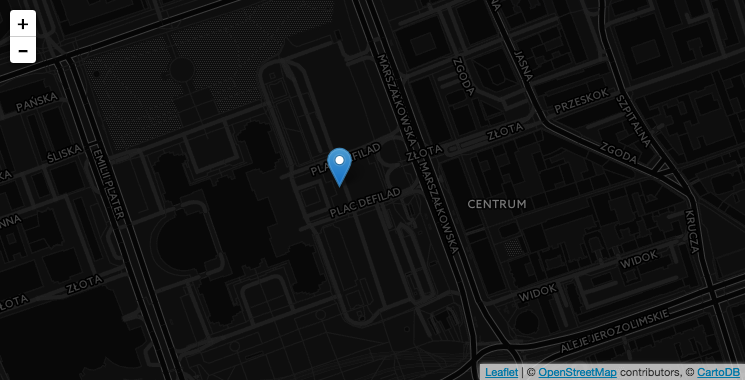
\includegraphics[width=10cm]{images/warsaw-center}
  \caption{Prezentacja punktu o współrzędnych 52.232222, 21.008333 - centrum Warszawy - na mapie}
  \label{fig:warsawCenter}
\end{figure}


Za obszar do obliczenia powierzchni Warszawy przyjąłem koło o podanym wcześniej punkcie centralnym i promieniu obliczonym na podstawie powierzchni Warszawy\cite{WarszawaWiki}. Takie obliczenia powinny być wykonywane na przybliżonym kształcie Ziemi — elipsoidzie. Jednak ze względu na statystyczne przeznaczenie dokładności potrzebnych informacji, przyjmuję, że kształtem obszaru tych obliczeń jest płaszczyzna. Więc wzór wygląda następująco:
\[ A=\pi*r^2 \]

Gdzie A to powierzchnia Warszawy, a natomiast r to szukany promień okręgu. Po odpowiednim przekształceniu wzoru i późniejszym podstawieniu \textit{517,24 km\textsuperscript{2} (1.01.2016)}\cite{WarszawaWiki} pod symbol A, otrzymujemy promień — r - o wielkości 12,8313km.


\begin{figure}[h!]
  \centering
    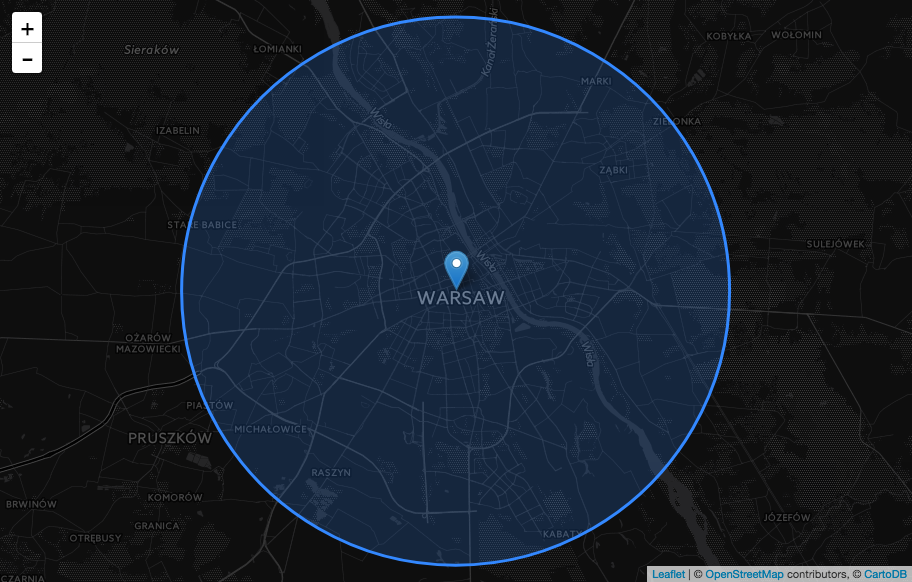
\includegraphics[width=10cm]{images/warsaw-10km-radius}
  \caption{Prezentacja koła o promieniu 12,8313km o środku w punkcie o współrzędnych 52,232222, 21,008333 na mapie}
  \label{fig:warsaw10kmRadius}
\end{figure}

\subsection{Statystyka}
Chcąc szacować ilość sieci bezprzewodowych w Warszawie, trzeba zacząć od ludności. Na stronie internetowej Urzędu Statystycznego w Warszawie stan ludności wynosił 1 753 977 osób (stan na dzień 31.12.2016). Dodatkowo w Warszawie funkcjonowało 424 195 przedsiębiorców. Posiłkując się informacją o przeciętnej liczbie osób w gospodarstwie domowym w województwie mazowieckim w kategorii miasta — wynosił 2,42.\cite{PrognozaGospodarstwGUS} Dzieląc ludność przez ilość przeciętnej ilości osób w gospodarstwie domowym, dostaniemy 724 784 gospodarstwa domowe w Warszawie. Na podstawie tych wartości możemy szacować, że 395 350 (93,2\%)\cite{SpoleczenstoInformacyjneGUS} przedsiębiorców oraz 548 662 (75,7\%) gospodarstwa domowe, które posiadają łącza szerokopasmowe, prawdopodobnie również posiadają przynajmniej jedno urządzenie oferujące sieć bezprzewodową. Daje to końcowy szacunek w okolicach \textbf{944 012} punktów bezprzewodowego dostępu do internetu.

\subsection{Na podstawie sieci bezprzewodowych}
W przypadku algorytmu estymującego lokalizację użytkownika na podstawie zarejestrowanych sieci bezprzewodowych musimy rozważyć wiele czynników takich jak:

\begin{itemize}
    \item urządzenia wypożyczone konsumentom — dostawcy usług telekomunikacyjnych nierzadko przywracają sprawne urządzenia do kolejnego klienta bez zmiany identyfikatorów sprzętowych
    \item mobilne hotspoty — smartfony mają możliwość tworzenia punktów dostępu dla innych urządzeń. Są też dedykowane rozwiązania rozdawane do abonamentów przez operatorów telekomunikacyjnych, takie jak Huawei MIFI.
    \item migracja ludności — na własnym przykładzie mogę powiedzieć, że od 3 lat mam ten sam Punkt Dostępu, a od kiedy go zakupiłem, przeprowadziłem się już 2 razy. Wielokrotnie miałem sytuacje, w których estymowana lokalizacja z Google, pokazywała okolice mojego poprzedniego zamieszkania. Szczególnie przy drugiej przeprowadzce.
\end{itemize}
%zdjęcie orange funbox
% zdjęcie mifi?
% zdjęcie routera ASUS?

\section{Aplikacja internetowa}
Natomiast rolą aplikacji internetowej będzie geolokalizacja na podstawie podanych adresów MAC oraz siły sygnału widocznych sieci. Miejsce zapisu zebranych danych, import dużych danych, wizualizacja, analiza, zapytania na bazie

\subsection{Ruby}
Ruby jest obiektowo-funkcyjnym interpretowanym językiem. Posiada zaimplementowane Odśmiecanie pamięci (z ang. Garbage Collector). \textit{Ruby bazuje na wielu językach, takich jak CLU, Eiffel, Lisp, Perl, Python czy Smalltalk. Składnia jest zorientowana liniowo i oparta na składni CLU oraz, w mniejszym stopniu, Perla.}\cite{RubyWiki}

Ruby został stworzony przez Yukihiro Matsumoto w 1995 roku. Od tego czasu doczekał się wielu poprawek i optymalizacji. Jest to też jeden z niewielu języków, który posiada wiele interpreterów spośród których najbardziej popularnymi implementacjami obecnie są:
\begin{itemize}
    \item MRI (Matz's Ruby Interpreter) - jest wyjściową implementacją i jest de facto specyfikacją języka
    \item JRuby - w większości napisany w Javie. Osiągnął dosyć dużą popularność, ze względu na dobrą zgodność z oryginalną specyfikacją przy większej wydajności.
    \item Ruboto - Nakładka na JRuby, która pozwala tworzyć aplikacje na Androida.
    \item RBX (Rubinus) - Oparty na projekcie maszyny wirtualnej Smalltalk-80
    \item RubyMotion - komercyjna implementacja na iOS, Mac OS X oraz Android
\end{itemize}

Wiele implementacji interpreterów. Przejrzysty i czytelny kod, który czyta się prawie jak naturalny język angielski. Spowodowały, że w latach 2008-2012 był najpopularniejszym językiem na GitHub.\cite{RubyStats2015} Niestety w kolejnych latach jego popularność spadała. W 2013 był drugi, w 2014 i 2015 był trzeci\cite{RubyStats2015}, w 2016 był już szósty i tak jest do dziś.\cite{GithutStats2017}

\subsubsection{Ruby on Rails}
Ruby on Rails jest zestawem bibliotek, które tworzą szkielet (z ang. framework) do budowania aplikacji internetowych zgodnie ze wzorcem architektonicznym Model-Widok-Kontroler (MVC) oraz z paradygmatem projektowym (z ang. design paradigm) Konwencja-Ponad-Konfiguracją (z ang. Convention-Over-Configuration). Kolejną ideą jest \textit{Nie powtarzaj się} (z ang. Don't Repeat Yourself) - sednem tej idei jest modularyzacja i poprawna strukturyzacja kodu. Dzięki takiemu podejściu kod aplikacji jest łatwiej czytać, modyfikować i testować.

%Warto jeszcze wspomnieć o standardach, które rządzą światem kontrolerów są to CRUD i REST. Pierwszy opisuje podstawowe operacje, które można wykonywać na

Połączenie dużej refleksyjności Rubiego, świetnej biblioteki ORM, czystej i zorganizowanej struktury plików, która dzięki konwencji, w każdym projekcie jest zawsze taka sama, to stworzyło jedno z najbardziej lubianych i najlepiej ocenianych pod względem produktywności środowisk do wytwarzania aplikacji internetowych.

Ze względu na bardzo kosztowną naturę powstawania aplikacji internetowych opartych na rozwiązaniu Ruby on Rails, popularność tej technologii w morzu internetu jest niszowa.\cite{TrendsBuiltWithRails}

\begin{table}
\caption{Użycie Ruby on Rails w internecie}
\label{table:rubyusage}
\begin{tabular}{ |l|l|l|  }
\hline
Kategoria & Liczba wykrytych z liczbą wszystkich & Procent \\
\hline
\hline
Top 10 tys. na postawie Quantcast & 558 z 10 000 & 5,6\% \\
\hline
Top 100 tys. na postawie Quantcast & 3 415 z 100 000 & 3,4\% \\
\hline
Cała baza builtwith.com & 1,162,698 z 370,442,435 & 0,3\% \\
\hline
\end{tabular}
\end{table}

Jak widać z Tablicy \ref{table:rubyusage} z tego rozwiązania korzystają aplikacje internetowe, które są oceniane wysoko w rankingu Quantcast. Strony takie potrzebują wysokiej jakości dopasowanych do ich potrzeb rozwiązań. Oczywiście nie zaprzeczam, że można korzystać z Ruby on Rails przy prostych potrzebach takich jak blogi z systemami zarządzania treścią lub przy kampaniach promocyjnych czy stronach produktów. Jednakże koszt powstania takiej strony internetowej jest niepotrzebnie duży. Przy takich potrzebach na rynku rozwiązań dużo lepszym rozwiązaniem byłby Wordpress, Joomla lub inny system do zarządzania treścią. Rozwiązania oparte na PHP mają mniejszy koszt infrastruktury w porównaniu do Ruby on Rails. Wsparcie techniczne i specjaliści są tańsi i łatwiej osiągalni.

\subsection{HTML}
Aplikacje internetowe nie istniałaby bez języka HTML. Ten już dość przestarzały język był wielokrotnie poprawiany i rozwijany na przestrzeni lat. Wciąż istnieje i nowoczesna jego odmiana w większości jest kompatybilna z poprzednimi wersjami.

\subsection{JavaScript}
Ze względu na ograniczenia interaktywności dokumentów HTML w pracy zostanie wykorzystany język JavaScript. W nowoczesnych aplikacjach internetowych jest to absolutnie normalne, że wykorzystuje się ten język do poprawienia użyteczności i ergonomiczności aplikacji. Pozwala tworzyć bardziej responsywne interfejsy użytkownika i wymieniać informacje z serwerem bez przeładowywania całej strony internetowej.

Język obecnie przeżywa drugie narodziny ze względu na wytworzoną przez Google interpreter V8, który umożliwia uruchomienie JavaScriptu bez przeglądarki. Takie usamodzielnienie języka spowodowało wielki wybuch narzędzi konsolowych, wielu nowych bibliotek oraz szkieletów do budowania aplikacji (z ang. framework). Stał się nowoczesną technologią do wytwarzania aplikacji internetowych, ze względu na możliwość pisania kodu aplikacji po stronie przeglądarki i po stronie serwera w jednym języku. Pozwala to na mniejsze wymagania wobec programistów i tym samym powoduje lepszą znajomość języka.

% gry, edytory 3d, geolokalizacja

%\subsubsection{AJAX}

\subsubsection{JSON}
To struktura danych, która zrodziła się na podstawie JavaScriptu.\cite{JsonWiki} Stał się nieodłącznym elementem w komunikacjach z interfejsami programistycznymi aplikacji internetowych ze względu na większą czytelność w trakcie procesu rozwoju oprogramowania od rozwiązań takich jak XML czy HTML. Nie posiada zadeklarowanej struktury do przechowywania danych i między innymi dlatego tak często z niego się korzysta przy prostych komunikacjach typu AJAX. Implementacja generatorów oraz parserów do tego standardu znajduje się w większości języków programistycznych.

%\subsubsection{GeoJSON}
%Jest otwartym standardem opisującym proste geograficzne kształty.

\subsection{PostgreSQL}
Źródłowo otwarty system zarządzania obiektowo-relacyjną bazą danych. Dla twórców ważną ideą jest zgodność ze standardami oraz możliwość rozszerzania funkcjonalności poprzez różne dodatki. Posiada implementacje na wszystkie najpopularniejsze systemy operacyjne takie jak Windows, Linux oraz Unix. Postgres (w skrócie od słowa PostgreSQL) dąży do pełnej zgodności ze standardem ACID.\cite{PostgresWiki}

\section{Aplikacja mobilna}
Rolą aplikacji mobilnej będzie odpytywanie aplikacji internetowej o lokalizację w oparciu i zbierane informacje. Dodatkowo aplikacja będzie umożliwiała obserwacje lokalizacji sieci bezprzewodowych i przesyłanie tych danych do aplikacji internetowej.

\subsection{Android}
Źródłowo otwarty system operacyjny tworzony przez Google oparty na Linux-owym jądrze. Zaprojektowany z myślą o urządzeniach mobilnych takich jak telefony i tablety. Głównymi narzędziami użytkownika są gesty na wyświetlaczu dotykowym, ale mimo tego, system ma wsparcie dla klawiatur i myszek.\cite{AndroidWiki}

\subsection{Java}
Choć rdzeń systemu Android jest napisany w C++, to aplikacje i interfejs użytkownika jest napisany w Javie.\cite{AndroidWiki}

Java jest jednym z najpopularniejszych języków programistycznych na świecie. Zależnie od różnych statystyk, ale wg. serwisu GitHut jest to \textbf{drugie miejsce na świecie.}\cite{GithutStats2017} Początkowym hasłem twórców tego języka było \textit{Napisz raz, uruchom wszędzie} (z ang. \textit{write once, run anywhere}). Jest silnie typowana, obiektowa i kompilowana do kodu bajtów dla maszyny wirtualnej.\cite{JavaWiki}

\subsection{XML}
Gdy Android powstawał, standard XML był nieodłączną częścią Javy. Naturalne jest, że znalazł on miejsce jako pliki konfiguracyjne oraz pewnego rodzaju struktura dla widoków aplikacji systemu Android.

Standard ten jest coraz częściej wypierany przez JSON ze względu na kiepską czytelność i dużą pracochłonność przy ręcznym tworzeniu i modyfikowaniu struktury danych, ale mimo wszystko umiejętność pracy z XML jest nieodłącznym atrybutem programisty.

\subsection{SQLite}
Do tymczasowego przechowywania danych podczas zbierania informacji o lokalizacjach sieci bezprzewodowych ta plikowa baza danych jest rozwiązaniem pasującym tutaj idealnie. W wielu aplikacjach Androidowych jest to podstawowy wybór, gdzie pojawiają się relacyjne dane, które trzeba przechować lub filtrować.

\section{Teza}
Na podstawie przeprowadzonej analizy moja teza składa się z trzech części, które definiują kryteria, dla których nawigacja w warunkach miejskich może być skuteczna. Tezę uznam za potwierdzoną gdy, spełnione zostaną wszystkich części w stopniu przynajmniej minimalnym.

\subsection{Część pierwsza - precyzja geolokalizacji}
Urządzenie z zainstalowaną aplikacją mobilną umożliwi precyzyjne określenie lokalizacji w warunkach miejskich. Poziom precyzji, który uważam za minimalny do skutecznej nawigacji pojazdu samochodowego przy prędkości nieprzekraczającej 60 km/h to 50 metrów. Zmierzenie tej wartości zostanie wykonane przez porównanie pozycję z odbiornika GPS i porównanie z pozycją otrzymaną przez geolokalizację na podstawie sieci bezprzewodowych w zasięgu urządzenia.

\subsection{Część druga - szybkość geolokalizacji}
Urządzenie z zainstalowaną aplikacją mobilną umożliwi określenie lokalizacji z odpowiednią szybkością w warunkach miejskich. Szybkość geolokalizacji, którą uważam za minimalny do skutecznej nawigacji pojazdu samochodowego przy prędkości nieprzekraczającej 60 km/h to 5 sekund. Wartość ta będzie wynikać ze średniego czasu pomiędzy otrzymanymi wynikami geolokalizacji.

\subsection{Część trzecia - zagęszczenie sieci bezprzewodowych na terenie Warszawy}
Na terenie Warszawy zagęszczenie sieci bezprzewodowych powinno wynosić w okolicach 1 825 sztuk na kilometr kwadratowy. Taką wartość otrzymałem poprzez podzielenie \textbf{944 012} - szacowanej ilości sieci bezprzewodowych na terenie miasta Warszawa na podstawie statystycznych informacji o ludności, gospodarstwach domowych oraz informacji o dostępnie do internetu społeczeństwa — przez \textbf{517,24 km\textsuperscript{2}} - pole powierzchni miasta Warszawa. Oczywiście wartość ta będzie się różnić ze względu na różnorodność zabudowy Warszawy. Jednakże nie może być mniejsza niż 400 sztuk na kilometr kwadratowy, bo oznaczałoby to dokładność geolokalizacji na poziomie 50 metrów.

\chapter{Część praktyczna}
W rozdziale tym przedstawię proces utworzenia aplikacji internetowej oraz mobilnej. Omówię wyzwania oraz problemy, z którymi się spotkałem podczas implementacji. Na koniec przeprowadzę badania i wyciągnę wnioski które skonfrontuje z postawioną tezą.


\section{Aplikacja mobilna}
Implementację aplikacji mobilnej rozpocząłem od kreatora, w którym wybrałem opcję pojedynczego Activity. Na początku zaimplementowałem odpowiednie algorytmy skanujące sieci bezprzewodowe w zasięgu. W kolejnym kroku dodałem obsługę urządzenia GPS. Następnie stworzyłem tabelę w bazie danych aplikacji mobilnej z odpowiednią strukturą do przechowywania zebranych obserwacji sieci bezprzewodowych. Na koniec zaimplementowałem prezentację geolokalizacji uzyskanej z aplikacji internetowe oraz możliwość eksportu zebranych obserwacji lokalizacji sieci bezprzewodowych.

\subsection{Uprawnienia na Android}

Począwszy od Androida 6.0 (poziom API 23), użytkownicy przyznają uprawnienia do aplikacji podczas uruchamiania aplikacji, a nie podczas instalowania aplikacji. To podejście usprawnia proces instalacji, ponieważ użytkownik nie musi przyznawać uprawnień podczas instalowania lub aktualizacji. Daje to również użytkownikowi większą kontrolę nad funkcjonalnością aplikacji; Na przykład użytkownik może się zdecydować, czy udostępnić kamerę dostęp do aparatu, ale nie do lokalizacji urządzenia. Dodatkowo użytkownik może cofnąć uprawnienia w dowolnym momencie, przechodząc do ekranu \textit{Ustawienia aplikacji}.\cite{NewPermissionsModelInAndroid60}

Nowy system uprawnień wymaga dodatkowej uwagi twórców aplikacji mobilnych. Zanim

\subsection{Skanowanie sieci bezprzewodowych}
Klasycznym przykładem tego, jak Android został zaprojektowany, jest własnie skanowanie sieci bezprzewodowych. Aby uzyskać obiekty klasy ScanResults. Po pierwsze, musimy uzyskać instancję programu WifiManager. Następnie dziedzicząc po klasie BroadcastReceiver zaimplementować metodę, która dostanie powiadomienie o zakończeniu przetwarzania. Taki asynchroniczny odbiornik — WifiScanReceiver — rejestrujemy z parametrem WifiManager.SCAN_RESULTS_AVAILABLE_ACTION i wreszcie rozpocząć skanowanie przez metodę startScan() na instancji WifiManager.

\begin{minted}{java}
wifi_manager = (WifiManager) getApplicationContext().getSystemService(Context.WIFI_SERVICE);
wifi_scan_reciever = new WifiScanReceiver();
registerReceiver(wifi_scan_reciever, new IntentFilter(WifiManager.SCAN_RESULTS_AVAILABLE_ACTION));
wifi_manager.startScan();
\end{minted}

I tu niespodzianka, bo w Androidzie nie mamy możliwości zaparametryzowania, że chcemy uzyskiwać wyniki o zeskanowanych sieciach w sposób ciągły. Musimy więc w naszym WifiScanReceiver zlecić ponowne skanowanie zaraz po otrzymaniu wyniku ostatniego skanowania. Tutaj jeszcze dodałem małe sprawdzenie, czy mamy aktualne współrzędne geograficzne do zapisania lokalizacji.

\begin{minted}{java}
private class WifiScanReceiver extends BroadcastReceiver {
        public void onReceive(Context context, Intent intent) {
            wifi_manager.startScan();
            if( last_location != null && ( (1000*10) > Calendar.getInstance().getTime().getTime() - last_location.getTime())){
                List<ScanResult> wifiScanList = wifi_manager.getScanResults();
                for (ScanResult wifi : wifiScanList) {
                    if( wifi.SSID.contains("_nomap") || wifi.SSID.contains("_optout") ){
                        wifiScanList.remove(wifi);
                    }
                }

                JSONArray array = new JSONArray();
                if (wifiScanList.size() == 0) {
                    wifis.add(getString(R.string.no_networks));
                } else {
                    ActiveAndroid.beginTransaction();
                    try {
                        for (ScanResult wifi : wifiScanList) {
                            WifiObservation wifiObservation = new WifiObservation(wifi, last_location);
                            array.put(wifiObservation.toJson());
                            wifiObservation.save();
                        }
                        ActiveAndroid.setTransactionSuccessful();
                    } finally {
                        ActiveAndroid.endTransaction();
                    }
                    runJavascript("geolocateByWifis("+array.toString()+")");
                }

            }
        }
    }
\end{minted}
W powyższym kodzie źródłowym widzimy usuwanie wyników zeskanowanych sieci z określonymi dopiskami. Wiąże się to z faktem, że Google zaproponowało dopisywanie do końca nazwy sieci \_nomap (z ang. nie mapuj), aby ich rozwiązania nie zbierały informacji o lokalizacji danych sieci bezprzewodowych.\cite{GoogleNomap} Dodatkowego zamieszania dorzuciła firma Microsoft, gdzie dla swoich rozwiązań zaproponowali \_optout (z ang. wypisz mnie).\cite{MicrosoftOptout}

\subsubsection{Problem z określeniem kierunku sygnału}
Nie jest możliwym stwierdzenie, z jakiego kierunku przyszedł sygnał sieci bezprzewodowej. Powoduje to, że zbieranie informacji o lokalizacjach sieci bezprzewodowych jest skazane na dużą niedokładność. Konkretniej spowoduje to umiejscowienie wszystkich sieci bezprzewodowych na pozycji telefonu dla algorytmów bardzo prymitywnych Np. na środku ulicy lub na chodniku. Bardzo dobrze to widać na /refs{fig:poor-scan-result}

\begin{figure}[h!]
  \centering
    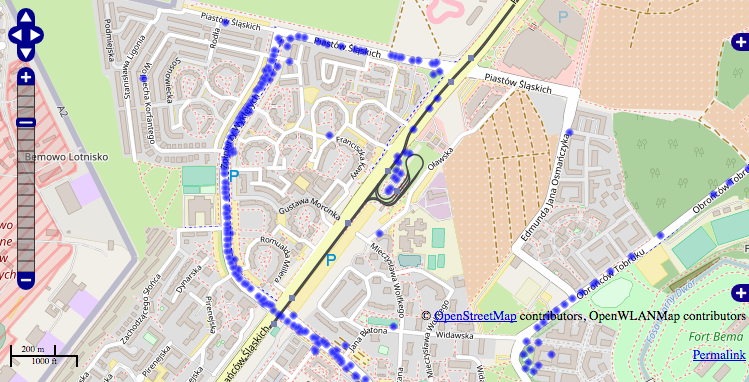
\includegraphics[width=10cm]{images/poor-scan-result}
  \caption{Prezentacja lokalizacji sieci bezprzewodowych na mapie - algorytm primitywny}
  \label{fig:poor-scan-result}
\end{figure}

Rozwiązaniem lepsze, ale droższe byłoby użycie kilku urządzeń, najlepiej z antenami kierunkowymi, dzięki czemu moglibyśmy stwierdzić czy stacja bazowa znajduje się po lewej stronie ulicy, czy po prawej na podstawie siły sygnału.
Dzięki technologii MIMO można określić, z którego kierunku przyszedł sygnał na jednym urządzeniu. Ze względu na denormalizację obserwacji sieci bezprzewodowych jesteśmy w stanie estymować kierunek, z którego przyszedł sygnał o ile mamy kilka zarejestrowanych skanów z różnymi siłami i lokalizacjami.


\subsection{Określanie lokalizacji urządzenia}
Do obsługi lokalizacji urządzenia poprzez GPS wykorzystałem bibliotekę — SmartLocation. Użycie prostego interfejsu biblioteki zaoszczędziło dużo czasu, który musiałbym poświęcić na zapoznawanie się z dokumentacją klas i interfejsów dotyczących nawigacji w Androidzie.

\begin{minted}{java}
public void startGpsListener(){
    SmartLocation.with(this).location().config(LocationParams.NAVIGATION).continuous().start(gps_location_listener);
}
private class GpsLocationListener implements OnLocationUpdatedListener {
    @Override
    public void onLocationUpdated(Location location) {
        last_location = location;
    }
}
\end{minted}

Sam proces uzyskania informacji o lokalizacji urządzenia jest asynchroniczny. Aby zniwelować efekt asynchroniczności, utworzyłem lokalną zmienną w ramach widoku, do której zapisuję ostatnią otrzymaną pozycję z SmartLocation. Do uzyskania najdokładniejszej pozycji skorzystałem z funkcji trybu nawigacji (z ang. navigate) z parametrem pracy ciągłej (z ang. continious). Trzeba pamiętać, że takie ustawienie jest niekorzystne dla czasu pracy na baterii, ale gwarantuje to najświeższą informację o współrzędnych urządzenia.

\subsection{Baza danych}
Teraz gdy już mamy wyniki skanowania sieci bezprzewodowych i lokalizację urządzenia, to jesteśmy w stanie zapisać wyniki do bazy danych aplikacji mobilnej — aby potem przesłać do aplikacji internetowej — dla lepszej precyzji określania lokalizacji sieci bezprzewodowych, a tym samym użytkownika.

Wybrałem bibliotekę ActiveAndroid jako ORM ze względu na swoje podobieństwo do ActiveRecord ze świata języka programowania Ruby oraz ze względu na użycie bazy SQLite, która jest popularnym rozwiązaniem do przechowywania danych na Androidzie. Stosując się do dobrych praktych twórców tej biblioteki, umieściłem tworzenie obserwacji w transakcji:

\begin{minted}{java}
ActiveAndroid.beginTransaction();
try {
    for (ScanResult wifi : wifiScanList) {
        WifiObservation wifiObservation = new WifiObservation(wifi, last_location);
        wifiObservation.save();
    }
    ActiveAndroid.setTransactionSuccessful();
} finally {
    ActiveAndroid.endTransaction();
}
\end{minted}

Po raz kolejny podjąłem decyzję o denormalizacji danych. Dane takie będą zajmować więcej miejsca, ale umożliwią na dokładniejsze lokalizowanie miejsca, w którym jest umiejscowiony punkt dostępu. Wszystkie dane będą zapisane w pojedynczej tabeli.

\begin{table}
\caption{Kolumny i typy przechowywania danych wraz z ich znaczeniem}
\label{table:dbscheme}
\begin{tabular} { |l|l|p{7cm}|  }
\hline
Typ & Nazwa & Znaczenie (opcjonalne) \\
\hline
\hline
String & ssid & \\
\hline
String & bssid & \\
\hline
int & signal_level & Wykryty poziom sygnału w dBm, znany również jako RSSI.\cite{scanResultAndroidDocs} \\
\hline
String & capabilities & Opisuje schematy uwierzytelniania, zarządzania kluczami i szyfrowania obsługiwane przez punkt dostępu.\cite{scanResultAndroidDocs} \\
\hline
Date & observed_at & Data i czas o sieć została zeskanowana \\
\hline
int & channel_frequency & Częstotliwość zeskanowanej sieci \\
\hline
double & latitude & Szerokość geograficzna pozycji, w której sieć zeskanowano \\
\hline
double & longitude & Wysokość geograficzna pozycji, w której sieć zeskanowano \\
\hline
Date & geolocated_at & Data i czas otrzymania informacji o współrzędnych geograficznych urządzenia \\
\hline
float & geolocation_accuracy & Dokładność współrzędnych geograficznych pozycji w któ®ej sieć zeskanowano \\
\hline
boolean & is_exported & Informacja o tym, czy sieć została wyeksportowana do aplikacji internetowej \\
\hline
\end{tabular}
\end{table}

Konstruktor klasy WifiObservation przyjmujący zeskanowaną sieć oraz ostatnią lokalizację zaimplementowałem następująco:
\begin{minted}{java}
public WifiObservation(ScanResult scanResult, Location location){
    super();
    this.ssid = scanResult.SSID;
    this.bssid = scanResult.BSSID;
    this.signal_level = scanResult.level;
    this.capabilities = scanResult.capabilities;
    this.channel_frequency = scanResult.frequency;

    this.observed_at = new Date();

    this.latitude = location.getLatitude();
    this.longitude = location.getLongitude();
    this.geolocated_at = new Date(location.getTime());
    this.geolocation_accuracy = location.getAccuracy();

    this.is_exported = false;
}
\end{minted}

\subsection{Prezentacja danych — mapa}

% dodałem flagę "android wake lock flag" żeby ekran się nie usypiał
% trzeba było włączyć CORS

\chapter*{Słownik pojęć}

\newcommand{\entry}[2]{\textbf{#1}\ $\bullet$\ {#2}}

\entry{ORM}{skrótowe oznaczenie dla "mapowanie obiektowo-relacyjne" (od angielskiego Object-Relational Mapping).}

\entry{Punkt dostępu (od ang. Accesspoint)}{Stacja bazowa WIFI.}
\entry{Aplikacja internetowa}{Aplikacja WWW/HTTP (webowa)}
\entry{SSID}{Nazwa punktu dostępu}
\entry{BSSID}{Mac Address}
\entry{Interfejs}{Międzymordzie}
\entry{Klastrowanie}{Zadaniem klastrowania jest pogrupowanie zbioru obserwacji w klastry tak, aby w ramach klastra obserwacje były do siebie jak najbardziej podobne, a jednocześnie jak najbardziej różne od obserwacji w innych klastrach.}
%https://eduwiki.wmi.amu.edu.pl/klastrowanie

\entry{Kanał (w kontekście sieci przezprzewodowych i punktów dostępów)}{WIFI operuje na określonych częstotliwościach. W przypadku 802.11g jest ich 14. Te poszczególne częstotliwości nazywamy kanałami.}

\entry{wardriving}{"zbieranie" jak najwiekszej ilosci sieci wifi.}
%https://en.wikipedia.org/wiki/Wardriving

\entry{MIMO (od ang. Multiple-Input-Multiple-Output)}{rozwiązanie w którym karta sieciowa posiada wiele wyjść i wiele wejść, przez co można nadawać i odbierać na specyficznym Wejściu/Wyjściu które posiada lepsze parametry komunikacji}

\entry{denormalizacja}{jest to wprowadzenie kontrolowanej nadmierności do bazy danych w celu przyśpieszenia wykonywania na niej operacji (np. obsługiwania zapytań); dzięki denormalizacji bazy unika się kosztownych operacji połączeń tabel}
%https://pl.wikipedia.org/wiki/Denormalizacja_bazy_danych




%\addcontentsline{toc}{chapter}{Literatura}

\listoftables

\bibliographystyle{abbrv}
\bibliography{bibliografia}

\end{document}
